\documentclass[11pt, table, dvipsnames]{beamer}
%\documentclass[11pt,handout]{beamer}
\usepackage{xcolor}
\usepackage[all]{xy}

\usepackage{hyperref}
 \title[Visual Text Analysis Hackathon]{Visual Text Analysis Hackathon}
\author{Paul Nulty}
%\institute % (optional)
%{
%  Department of Methodology, \\
%  London School of Economics and Political Science, \\
%  \vspace{2 mm}
%  \textit{QUANTESS} ERC Project 
%}
 
\date % (optional)
{LSE \\ 
24th March 2016}


\graphicspath{ {./graphics/} }
\definecolor{customBlue}{rgb}{0.9,0.9,0.95}
\begin{document}

\begin{frame}%<handout:0>
\titlepage
s\end{frame}

\begin{frame}
  \frametitle{Two dimensional Correspondence Analysis}
  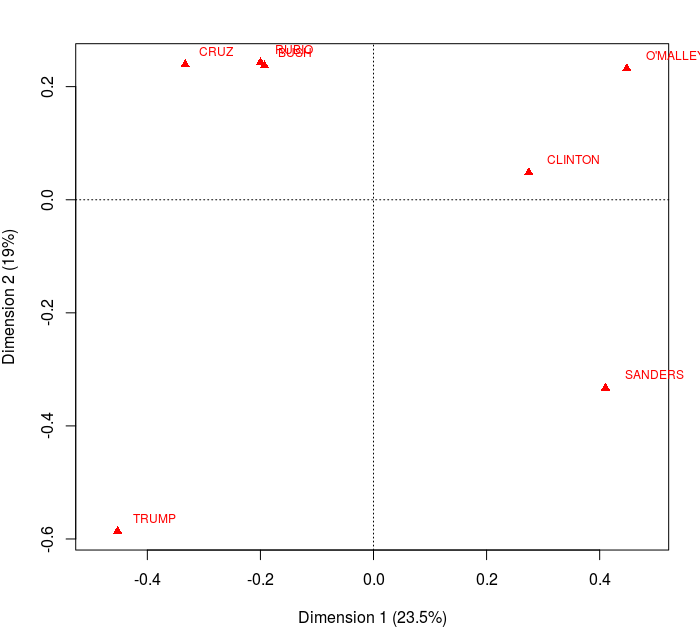
\includegraphics[scale=0.35]{2DCA}\\
\end{frame}


\begin{frame}
  \frametitle{Comparison Cloud}
 \begin{itemize}
  \item Treat words with positive, negative weights on a dimension as two documents
  \item Size: magnitude of difference from average rate of occurrence
  \item See \texttt{?comparison.cloud}
  \end{itemize}
\end{frame}

\begin{frame}
  \frametitle{Dimension One}
  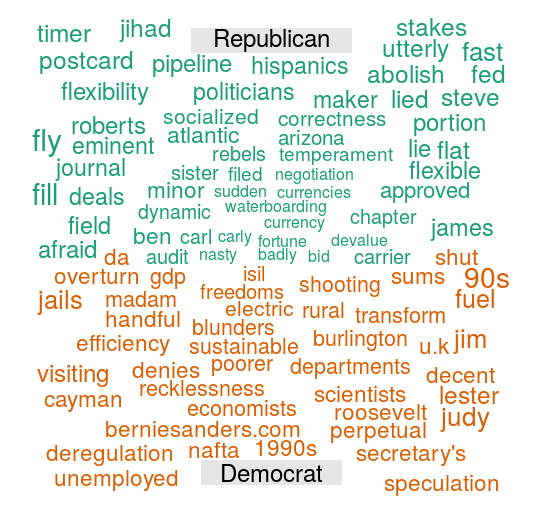
\includegraphics[scale=0.45]{Dim1.png}\\
\end{frame}

\begin{frame}
  \frametitle{Dimension Two}
  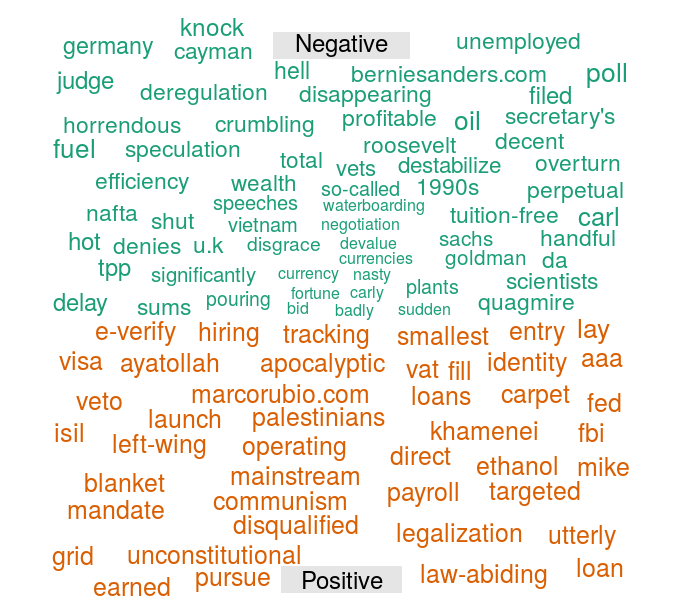
\includegraphics[scale=0.40]{Dim2.png}\\
\end{frame}

\begin{frame}
  \frametitle{Alternative: regularised regression, words as predictors} 
  \begin{itemize}
  \item glmnet elastic net, trigrams, bigrams and unigrams
  \item Keep features occurring more than five times
  \item Five-class multinomial logistic model for speaker
  \item 3195 parameters (approx. 800 nonzero at min CV error), 1470 documents, cross. val. accuracy: 78.7\%
  \item
  \item binomial model for party
  \item 3195 parameters (approx. 1481 nonzero at min CV error), 1470 documents, cross. val. accuracy: 89.5\% 
  \end{itemize}
\end{frame}

\begin{frame}
  \frametitle{Party regression model}
\begin{figure}
\centering
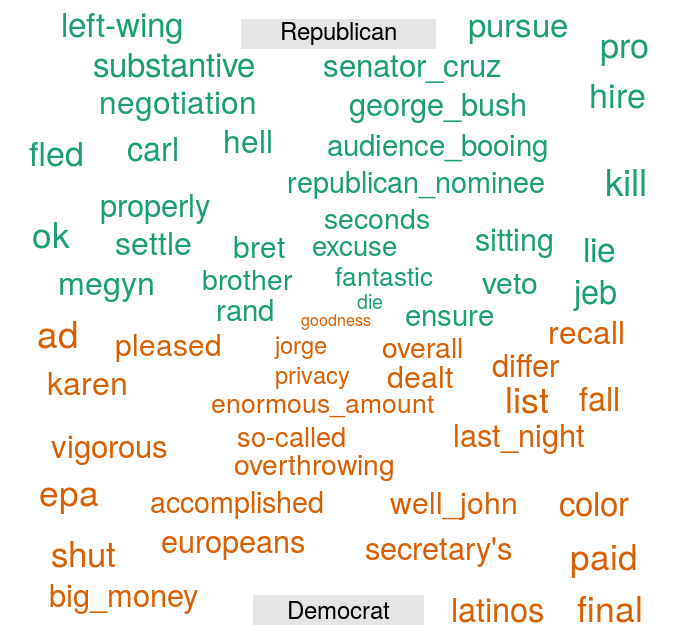
\includegraphics[width=0.7\linewidth]{../figs/partyCoefs}
\end{figure}
\end{frame}


\begin{frame}
  \frametitle{Tools} 
  \begin{itemize}
  \item General R: RStudio, dplyr
  \item Models: ca, glmnet
  \item Text: quanteda 
  \item Vis: shiny, wordcloud::comparison.cloud
  \end{itemize}
\end{frame}

\begin{frame}
  \frametitle{thank you} 
  \begin{itemize}
  \item Thank you for your attention
  \item Code available \url{https://github.com/pnulty/text-hackathon-2016}
  \end{itemize}
\end{frame}

\end{document}
